% Cole Nielsen niels538@umn.edu
% EE 2002 Spring 2015
% Formal Lab Report 1

%----------------------------------------------------------------------------------------
%	PACKAGES AND DOCUMENT CONFIGURATIONS
%----------------------------------------------------------------------------------------

\documentclass[12pt]{article}

\usepackage{circuitikz}
\usepackage{graphicx}
\usepackage{subcaption}
\usepackage[top=1in, bottom= 1in, left=1in, right= 1in]{geometry}
\setlength\parindent{0pt}
\usepackage{fancyhdr}
\pagestyle{fancy}
\usepackage{textcomp}
\usepackage{tikz}
\usepackage{siunitx}
\usepackage{placeins}
\usepackage{titlesec}
\usepackage{cancel} 
\usepackage{tikz}
\usetikzlibrary{shapes.geometric, arrows}
\tikzstyle{box} = [rectangle, rounded corners, minimum width = 3cm, minimum height = 1cm, text centered, draw = black]
\tikzstyle{arrow} = [thick,->,>=stealth]
\usepackage{placeins}

%----------------------------------------------------------------------------------------
%	DOCUMENT INFORMATION
%----------------------------------------------------------------------------------------

\title{Labs 1-4 \\Formal Report\\ \vspace{0.3 in} EE 4301}

\author{Cole \textsc{Nielsen}} 
\date{Fall 2015}

\newcommand{\mymeter}[2]{   	% #1 = name , #2 = rotation angle
 \begin{scope}[transform shape,rotate=#2]
   \draw[thick] (#1)node(){$\mathbf V$} circle (11pt);
   \draw[rotate=45,-latex] (#1)  +(-17pt,0) --+(17pt,0);
 \end{scope}
}

\begin{document}
\maketitle 

\pagebreak
%---------------------------------------------------------------------------------------
%----------------------------------------------------------------------------------------
%	Introduction
%----------------------------------------------------------------------------------------
\section{Introduction}
%
The Field Programmable Gate Array, or FPGA, is a programmable logic device which can be used to implement virtually any digital circuit in actual hardware. A programmable logic device (PLD) refers to a hardware device that can  be programmed to perform some digital function, much like a computer is programmed to execute instructions. They consist of many logic gates or circuits that implement logical function, that are initially unconnected and unconfigured. When they are programmed, the gates are connected together in a way that builds up a digital circuit. Unlike a computer, which is a fully implemented digital circuit that works out of the box, PLD's have no function and will do nothing until programmed. The process of programming a PLD involves creating a hardware description, which is just something that describes the circuit design. The hardware description can be done many ways, commonly being done by creating a schematic of the circuit entered into PLD design software, or using a Hardware Description Language (HDL). A HDL is a computer language that describes circuits and digital systems textually. For example, gates can be represented as an identifier with a certain syntax and variables for inputs and outputs. The most commonly used HDLs are VHDL and Verilog (Verilog was used in this lab). When a full hardware description is ready to be implemented into hardware, software tools are used to synthesize and compile the hardware description into an output (perhaps a mask for an IC, or a configuration "bitstream" for an FPGA) that implements the design in the target architecture/hardware. After this is done, the device being used can be programmed with that output, and the device should behave as the hardware description described.\\\par

Applying this to FPGA design, the design flow can be described in a high level with the following flow chart in \textit{Figure 1}. First, the design flow starts out with some sort of design requirement or specification, describing what the FPGA will need to do. Basic, high level idea of the design implementation should be forged at this point to guide the entry process. The following step, design entry, involves creating a hardware description of some digital system that implements the design requirements. This is often done with a HDL or schematic entry. When a complete design is entered, it needs to be verified to ensure it works. This is done in the next step, which is behavioral simulation. Behavioral simulation is a simulation of a description before synthesis, so it is a way of verifying if the digital design itself behaves as it should. The design should be tested with all expected input and state combinations if possible to make sure the design is functional. A design is verified this way by creating a test bench in Xilinix ISE and running it in a simulator, such as ISIM. Once the verification is successful, the design should be synthesized and implemented (routed onto the device). This part can be done automatically in Xilinx ISE. If so desired, the design can be manually routed with most FPGA design tools (FPGA editor in ISE), and timing parameters can be constrained (using Constraints Editor in ISE) so that the auto router places them to meet design specifications (if used). When this is done, the design should once again be verified, to make sure that the digital design was properly implemented in the FPGA. Logically sound designs often will not work if not implemented properly, due to timing issues in the chip, so this step is important. Within ISE, the timing parameters of the chip can be analyzed using the Timing Analysis tool, which gives a detailed report of a design's timing parameters. With the timing report, one can tune the constraint of the system to gain desired operation. When this appears to be good,the last step can be performed by generating the FPGA programming file, or the "bitstream", and loading it to the FPGA. Now, the device should be working as designed, however should be tested to ensure proper operation. If the design doesn't work after programming, the timing should be again verified and adjusted. If the design still doesn't operate properly, checking of the hardware decription should be done (if the fault has been concluded as not a timing issue).
\FloatBarrier
\begin{figure}[h!]
\begin{center}
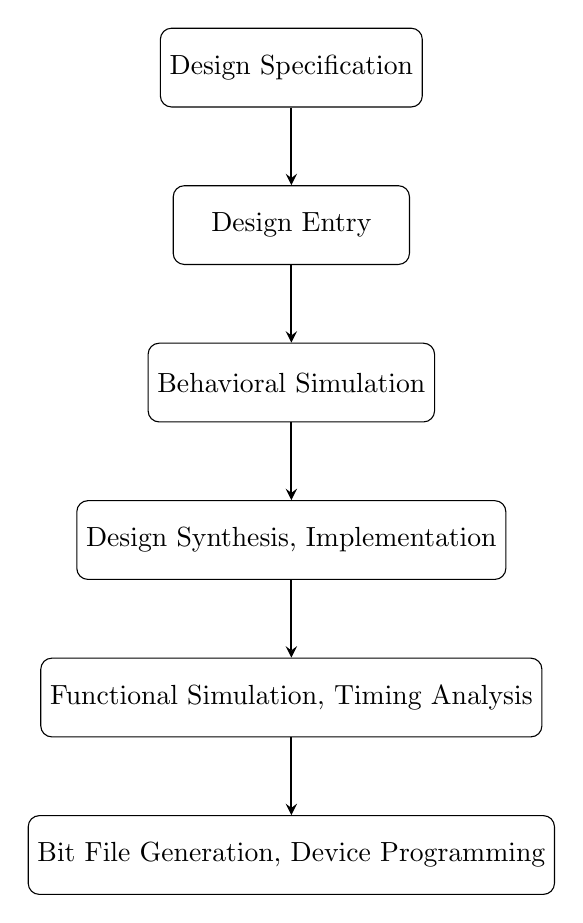
\begin{tikzpicture}[node distance = 2cm]
\node (design) [box] {Design Specification};
\node (entry) [box, below of=design] {Design Entry};
\node (simulation) [box, below of=entry] {Behavioral Simulation};
\node (synth) [box, below of=simulation] {Design Synthesis, Implementation};
\node (time) [box, below of=synth] {Functional Simulation, Timing Analysis};
\node (prog) [box, below of=time] {Bit File Generation, Device Programming};
\draw [arrow] (design)--(entry);
\draw [arrow] (entry)--(simulation);
\draw [arrow] (simulation)--(synth);
\draw [arrow] (synth)--(time);
\draw [arrow] (time)--(prog);
\end{tikzpicture}
\end{center}
\caption{Basic FPGA Design Flow}
\end{figure}
\FloatBarrier

Now understanding the operation and implementation of FPGA devices, it is easy to understand why FPGA design is useful. The first reason that should be noted is that implementing a digital hardware design is far easier and cheaper in lower quantities to do in an FPGA then fabricating a custom ASIC, as it mainly only requires the hardware design and then minimal work to implement the design to the FPGA. Another huge advantage of FPGAs (especially over ASICs) is that they are reprogrammable. If a design is faulty, one can easily go back, fix the hardware description, and then reprogram devices in the field (hence "field programmable"). This is not possible with ASIC designs, instead the chips would have to be refabricated, which is expensive. This makes FPGA designs inherently less risky, another advantage. A final aspect that makes FPGA design useful is that FPGAs can be made to do specific tasks far faster, efficient and with less latency than a microprocessor. This is because microprocessors are limited in the size of data they can operate on per cycle (often less than what is needed), and due to general-purpose architectures they generally need many cycles to achieve the operation being performed (to achieve specialized functions). On a FPGA, execution time can be minimized by creating specialized circuits for specific operations that can operate on more data at once, and then can compute the operation in fewer cycles (for example, a 32 bit microprocessor would take several cycles to add several 32 bit numbers, where as a FPGA could add all the numbers together at once in once cycle). Also, microprocessors will often have overheads due to handling interrupts, which may cause latency, where as FPGAs can be designed to process data in real time, and in parallel, so task can be done simultaneously, causing essentially no latency.
%----------------------------------------------------------------------------------------
%	Experiment
%----------------------------------------------------------------------------------------

\section{Design Flow}
In this section, the parts of the design flow are discussed in greater detail.
\subsection*{Design Entry}
Design entry begins with a design specification, which is a high level description of what the circuit needs to do. From the description, a circuit can be designed, by breaking it down into functional modules to implement this circuit. A top down approach to this may be to design a controller and a data path, and then break those modules into smaller modules until they can be described as circuits that can be entered either as a schematic  entry and then connected to form the greater design. Overall, from the specification, Verilog modules will be coded, in ISE using the build in editor, or as a schematic in the ISE schematic editor. When this is done, the result will be a collection of modules describing the device.
\subsection*{Behavioural Simulation}
When the hardware description is ready, the design needs to be simulated to verify that it is functional, atleast in a logical sense. It is important to verify the design itself separately from the design implemented in the FPGA because timing issues could cause a functional design to not work in a FPGA, which is hard to diagnose. If the design is known to work, but it doesn't run on a FPGA, it can be deduced that it is a timing problem. A simulation in ISE is prepared by creating a Verilog test bench file, which is essentially another Verilog module that outputs a series of stimuli into the DUT (device under testing). When a test fixture has been coded, the design and test fixture can be opened with a simulator, and in ISE this is ISIM. The simulator should show a waveform output for the stimuli for the set simulation time, and some output files containing that data. This output can be checked to make sure the design works.
\subsubsection*{Design Implementation}
A functioning hardware description can then be implemented into hardware using sythesis and placement tools. The synthesis of Verilog for FPGA implements the design into the FPGAs logic implementation, which typically involves many look up tables. In ISE this is done by the XST synthesizer. The design is then routed, which is the process of connecting the logic blocks implemented in the FPGA's architecture to each other to achieve satisfactory timing and operation. This can be done automatically in ISE, or manually with the FPGA Editor. The end result is output files containing the placement and implementation of the hardware description in the FPGA.
\subsection*{Timing Analysis/Functional Simulation}
When the design implementation is done, some additional verification can be performed before programming the FPGA to verify correct operation. In ISE, verification of timing is done using the Timing Analysis tool which generates a report of the implementations timing. The report can be reviewed, and if any parameters are not satisfactory, a constraint to the design's placement can be added in ISE's Constraint editor. Rerunning the placement step will result in a properly timed implementation if everything is corrected. The output of this step is the implementation of the design from the last step, but verified to have proper timing.
\subsubsection*{Programming}
With a implemented design known to function properly, the programming files for the FPGA can be generated and loaded to the FPGA. In ISE, the programming file is done by running "Generate Programming File" in the processes menu for the design. The output is a bitstream ".bit" file, which contains the necessary data to configure all the FPGA's look up tables, the routing fabric, IO modules and so on. Programming is performed by using a JTAG interface to load the bitstream directly into the FPGA, or into a EEPROM that can be read by the FPGA. The FPGA's memory is volatile, so everything written to it will be erased when powered off. An EEPROM (connected to the FPGA) is written with bitstream when the FPGA is desired to automatically program upon power-up without a JTAG programmer. For this lab, Digilent's Adept and a BASYS2 board was used to program a Xilinx Spartan 3E FPGA.
\section{Lab 1: Verilog Design Entry, Synthesis, and Behavioral Simulation File resource}
In this lab, a provided 4 bit adder subtracter design was implemented on a BASYS2 FPGA boards with ISE. The first step was to enter the given hardware design (design entry step) into ISE as two Verilog modules. First, a new project was made, and then a new verilog module was created, blank. The given code was then pasted into the editor for a full adder. A new module was added to the project, being a 4 bit adder-subtracter, and the code was again. Next, a behavioral simulation was performed by adding a new source (verification), being a Verilog test fixture. Verilog code was entered for the simulation, testing additions with no overflow, with overflow, subtractions with positive and negative results, and a subtraction with underflow. The results of the simulation is attached. After the simulation was found to be successful, then design moved into the implementation step. A Implementation Constraint File was added by adding a new source. The constraints file for the BASYS2 board was put in, an the pins were locked to the appropriate net variables of the design. Finally, the design was synthesized. The outcome of this lab was a understanding of how to enter, simulate and partially implement a FPGA design.
\section{Lab 2: Implementation and Timing Analysis File resource}
The objective of this lab was to perform the implementation of the design from lab 1. The first step of this was to route the design, which was automatically done by the auto-router in ISE. The placement of the design was viewed, however with FPGA editor to learn how to use the tool, and to observe how the device was laid out. Also, all output files of the routing were checked for any errors. Next, a timing analysis was performed on the design to verify that it functioned properly. It was found that the maximum pad to pad delay on this design for the Spartan 3E was approximately 10.5 ns. In order to reduce this time, Constraints editor was used to impose a maximum of 10 ns as a pad to pad delay. The design was rerouted and the maximum delay time was then found to be about 9.8ns (See the attached report), which is less then the specified value. This shows that designs can be tuned according to faults seen in the verification process. The overall outcome of this lab was a better understanding of the implementation step and verification process in FPGA design, as well as how to constrain designs according to the results of verification.
\section{Lab 3: Schematic Design Entry, Implementation, and Simulation File resource}
In this lab, the objective was to perform the design entry step using a schematic editor of ISE instead of Verilog. This shows that there are several ways to input a hardware description. This was performed in ISE by creating a new project and adding a schematic sheet. A full adder was created using logic gates, as shown on one of the attached print outs. The schematic was saved, and a symbol was made for the module so it can be used in higher level schematics. Another schematic module was added, and a four bit adder and subtracter was entered, using the full adder module created. This was saved. A Verilog test fixture was then created by adding another source, and the same series of stimuli used on the verilog version of the design was entered. The simulation was ran (behavioral simulation), and it was observed that the output (also attached) was then same as the verilog design, meaning this method of design entry works. Overall, it was learned hot to use schematic design entry, and that there are many ways to describe a design.
\section{Lab 4: Downloading to the Basys 2 Board File resource}
The final lab part was focused on the programming part of FPGA development. This was done by first generating a bitstream file in Xilinx by running "Generate a Programming File" in ISE for the design in processes. Digilent Adept was then used to upload the output programming file using the build in JTAG programming interface of the BASYS2 to the FPGA. The design was then tested by using the BAYSYS 2's built in switches and LEDs to verify the design works properly. Overall this lab taught the process to actually programming the device, and verifying functionality on the device.
%-----------------------------------------------------------------------------
%	Conclusion
%----------------------------------------------------------------------------------------
\section{Conclusion}
The FPGA design process can be summarized in a few parts. First is design entry, which is the creation of a circuit design from design requirements that implements those requirements. The next step is design verification, which checks if a design works properly through simulation. The next step is implementation of the design into the FPGA, which involves compiling the design into something that will work on the FPGA, routing out that and making sure the timing is correct. Finally, the completed design can be compiled into a programming file and loaded onto the FPGA for testing, then use.
\end{document}
